\section{Results}

\subsection{Pipeline performances}

The programs were run on a computer with an Intel Core i7-4790k CPU @ 4.0 GHz with 32 Gb of memory. The following histogram show the processing time of Quandenser pipeline, OpenMS and MaxQuant for the two data sets.

\begin{figure}[H]  %% CHANGE TO STYLE WHITE (NO BACKGROUND) + ta bort titel i plot + set_context('talk') (fonter)
  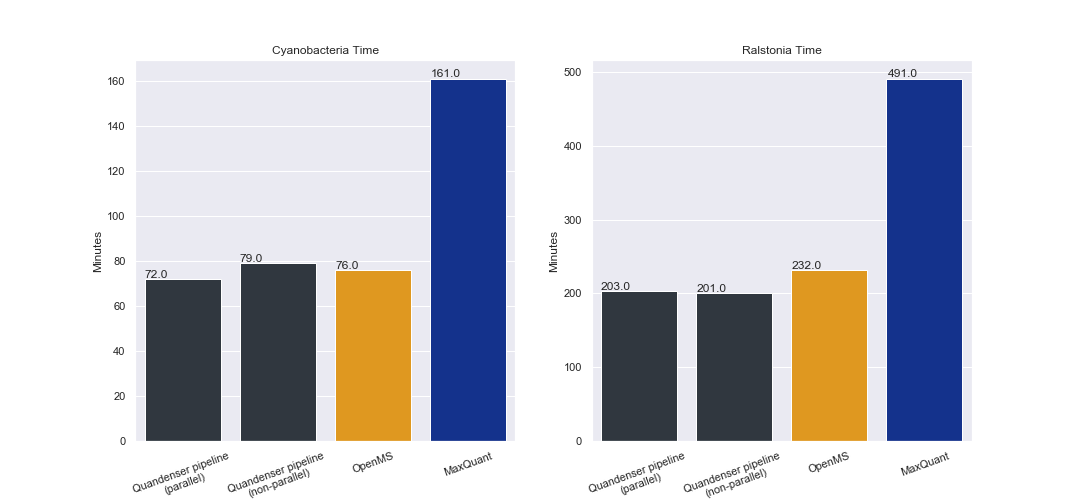
\includegraphics[width=\linewidth]{results/times.png}
  \caption{\textbf{Processing time on local computer (wall time)}. Note that \textit{parallel} Quandenser used a maximum of two forks (aka two processes in parallel), which was the maximum the computer could handle}
  \label{fig:processing-local}
\end{figure}
% Första meningen är bold (titel för bilden)
% Skriv om experimentet, vilka det är (left right) samt antal filer

\begin{figure}[H]
  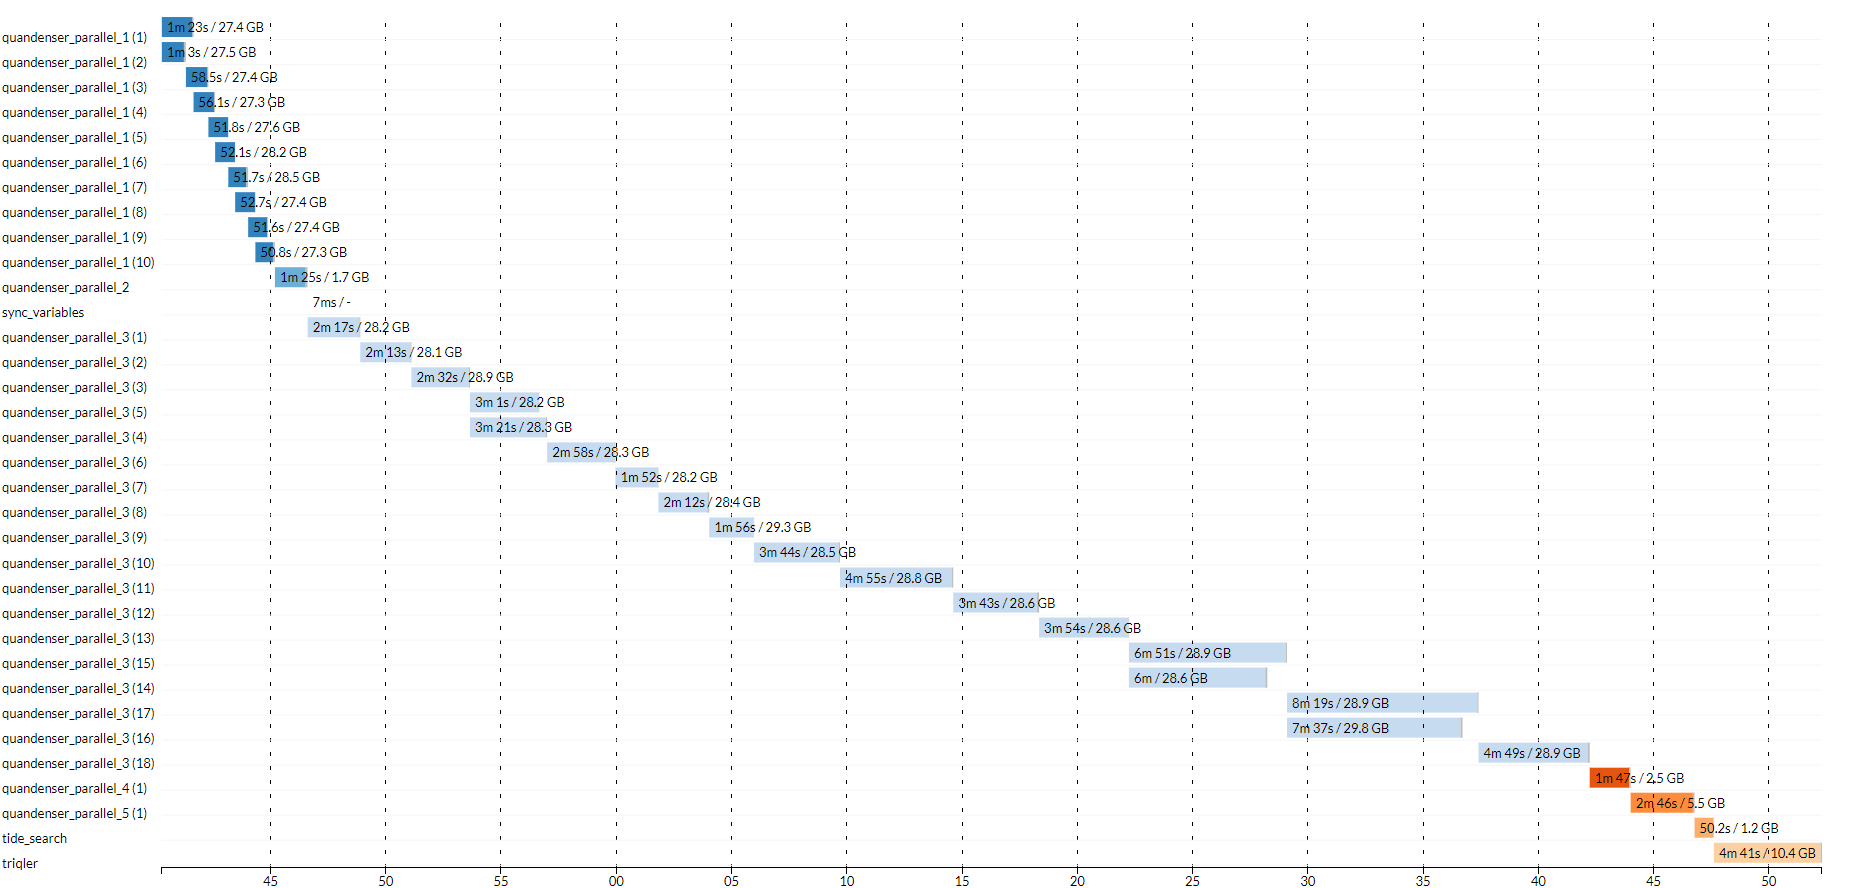
\includegraphics[width=\linewidth]{results/timeline-local.png}
  \caption{Timeline of parallel processing of the cyanobacteria data set on the local computer. Note that \textit{quandenser\_parallel\_1} is "fully" parallelizable while \textit{quandenser\_parallel\_3} is partially parallelized, following a minimum spanning tree explained in section \ref{ssec:quandenser-method}. The rest of the processes are non-parallelizable. A maximum of two forks was set (aka two processes in parallel)}
  \label{fig:timeline-local}
\end{figure}

\begin{figure}[H]
  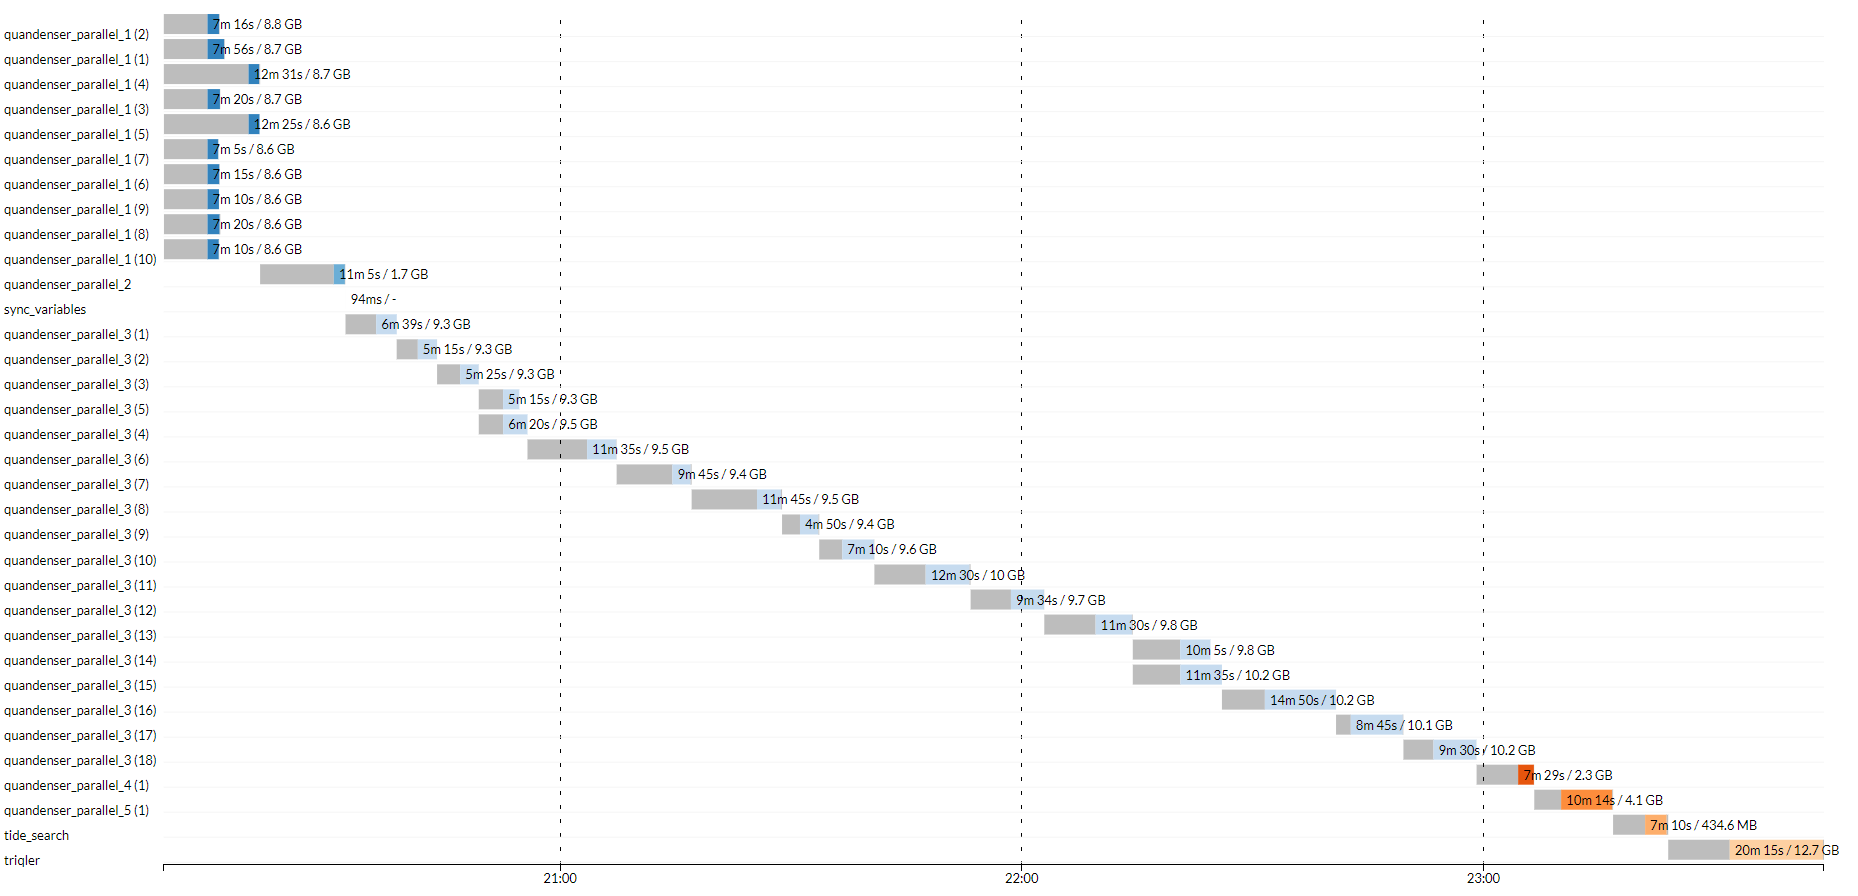
\includegraphics[width=\linewidth]{results/timeline-cluster.png}
  \caption{Timeline of parallel processing of the cyanobacteria data set on UPPMAX. The caption of figure \ref{fig:timeline-local} explains the processing names. The grey area of each bar represents SLURM queue time for each process. Unlimited amounts of processes was set, meaning no limit was set to the amount of parallelized processes possible}
  \label{fig:timeline-cluster}
\end{figure}

\subsection{Biological data}

The cyanobacteria experiment groups were divided in five groups; before dawn (A), after dawn (B), noon (C), before sunset (D) and after sunset (E) with two replicates each. From the cyanobacterial data set, each combination of experiment groups were compared to one another, i.e. all groups were compared to all other groups. For the ralstonia dataset, the same method applied.

For the cyanobacteria dataset, a total of 24 proteins between groups were found to be differentially expressed, which consisted of 10 unique proteins (shown in table \ref{table:cyano-proteins}). For the ralstonia dataset, a total of 760 proteins between groups were found to be differentially expressed, which consisted of 267 unique proteins. Due to the large amount of unique proteins found in the ralstonia data set, the ralstonia proteins were not analyzed.

\begin{center}
\begin{table}[H]
\caption{Quandenser pipeline cyanobacteria differentially expressed proteins, data gathered from NCBI gene search \cite{ncbi-search}}
\begin{tabular}{ l l }
\toprule
Protein & Function \\ \midrule
ssr3383 & Phycobilisome LC linker polypeptide \\ [0.5ex]
slr0083 & ATP-dependent RNA helicase \\ [0.5ex]
ssl2501 & Hypothetical protein \\ [0.5ex]
slr0473 & Phytochrome \\ [0.5ex]
sll1184 & Heme oxygenase \\ [0.5ex]
sll1214 & Magnesium-protoporphyrin IX monomethyl ester cyclase \\ [0.5ex]
sll1452 & Nitrate transport protein \\ [0.5ex]
slr2032 & Hypothetical protein \\ [0.5ex]
ssr1480 & RNA-binding protein \\ [0.5ex]
slr1739 & Photosystem II protein (PsbW) \\ \bottomrule
\end{tabular}
\centering
\label{table:cyano-proteins}
\end{table}
\end{center}

% Ta abundances, lägg i tidsaxis
\begin{figure}[H]
  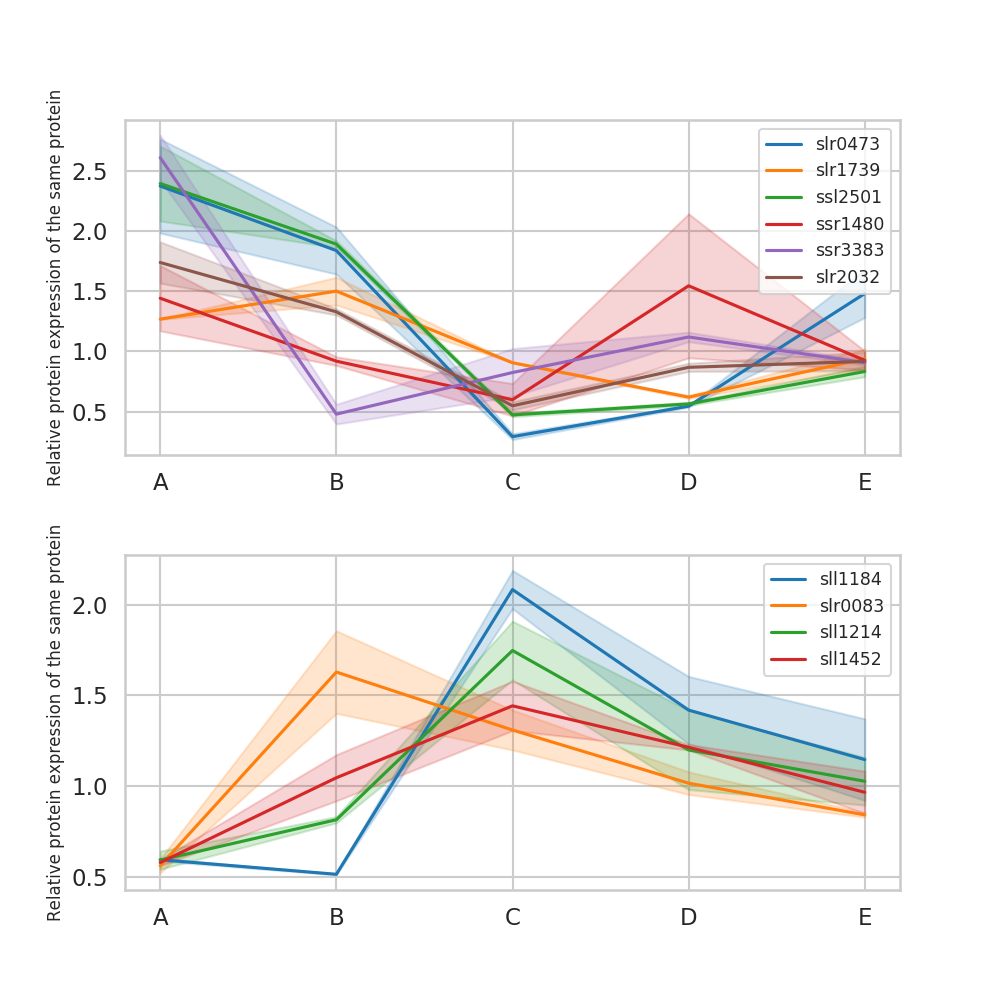
\includegraphics[width=\linewidth]{results/combined.png}
  \caption{Heatmap of fold changes between groups of the differentially expressed proteins. To interpret the plots, the comparison is \textbf{y}vs\textbf{x} where y is the group at the y-axis and x the group at the x-axis. If you were to look at the first row, second column, it would be the comparison of the log2 fold change between AvsB. A positive value would mean that group A has a higher expression that group B.}
  \label{fig:heatmap}
\end{figure}
